% This is an example of how to create a presentation in PDFLaTeX. 
% Matt Welsh, mdw@cs.berkeley.edu
% See http://www.cs.berkeley.edu/~mdw/proj/texslides for details.

% The basic document style is 'foils' from the FoilTeX package
\documentclass[20pt,landscape]{foils}
% These are my macros for creating slides
\usepackage{mdwslides}
\pdfoutput=11
% Basic things that we need are below
\usepackage[english]{babel}
\usepackage{hyperref}
\usepackage{color}
\hypersetup{
  pdfmenubar=true,
  pdftoolbar=true,
  pdfpagemode={None}
}
\usepackage{pause}
\usepackage{graphicx}
\usepackage[utf8]{inputenc}
\inputencoding{utf8}
%%%%%%%%%%%%%%%%%%%%%%%%%%%%%%%%%%%%%%%%%%%%%%%%%%%%%%%%%%%%%%%%%%%%%%%%%%%%

% Set headers
\MyLogo{Ole Aamot}
\rightfooter{\quad\textsf{\thepage}}

\begin{document}
\rm

\slide{}
\LogoOff

\vskip 1.5in
\begin{center}
  {\color{mdwblue}\Large\slingbold Free Software for Free Radio with GStreamer
    \vskip 11ex
    Ole Aamot
    \vskip 1ex
           {\small\trebucit ole@gnome.org}
           \vskip 1ex
                  {\mdwsmall\tt \url{https://www.gnome.org/~ole/GC2019.pdf}
                  }
  }
\end{center}

\slide{What is Free Radio?}

My presentation at the GStreamer Conference 2019 in Lyon, France as the
GNOME Radio developer and maintainer is about Civil Rights and Social 
Action with Free Software.

Live radio broadcasts covers events on every continent, every conflict, every human tragedy and triump in the world and Free Radio is about promoting news about human rights, peace and knowledge sharing between humans just like Free Software.

The title of my Bachelor of Science thesis at Oslo Metropolitan University in Norway is ``Public Internet Radio Client for Accessing Free Audio Maps in Countries with Free Speech'' available from \url{http://www.oleaamot.com/thesis/thesis.pdf}

GNOME Radio is the future Public Network Radio Software for Accessing
Free Audio Broadcasts from the Internet on GNOME after 5 years of work 
on GNOME Internet Radio (gnome-internet-radio-locator) since 2014 that
began at Norwegian Computing Center in 2002.

Live playback support implemented GStreamer is available in GNOME Radio.

\slide{Introduction}
\LogoOn

GNOME Internet Radio Locator (gnome-internet-radio-locator) is a Free
Software program that allows computer users to easily locate and
listen to radio programs on broadcasters on the Internet such as BBC,
KEXP and WMBR, as well as NASA's Third Rock Station and 113 other
Internet Radio stations broadcasting from many universities around the
world.

GNOME Internet Radio Locator (gnome-internet-radio-locator) is
developed for the GNOME 3.34 desktop and requires GStreamer
(\url{https://gstreamer.freedesktop.org/}) and the codec plugins to be
installed for live audio playback.  The player code was based on code
from gst-play written by Tim-Philipp Müller, Sebastian Dröge and
Brijesh Singh.  (See
\url{https://gitlab.gnome.org/GNOME/gnome-internet-radio-locator/blob/master/src/gnome-internet-radio-locator-player.c})

GNOME Internet Radio Locator (gnome-internet-radio-locator) is not
officially a part of GNU or GNOME, but using the *.gnome.org
infrastructure
on\\ \url{http://gitlab.gnome.org/GNOME/gnome-internet-radio-locator}
and\\ \url{https://download.gnome.org/sources/gnome-internet-radio-locator/}

\slide{Why do I write gnome-internet-radio-locator?}

\begin{list1}
\item I am a supporter of
  \begin{list2}
  \item Free Radio
  \item Free Software
  \item Free Speech
  \end{list2}
\item I want to give something back to the Free Software community
\item Internet Radio is a free Internet resource
\item Many Universities run non-profit Internet radio stations
\end{list1}

\slide{History of gnome-internet-radio-locator}

\begin{list1}
\item 2019
  \begin{list2}
  \item gnome-internet-radio-locator version 2.1.1 was released on October 24
    \begin{list3}
    \item Fancy City Color Markers   
    \item 117 Internet Radio Stations from 90 Major World Cities
    \item Graphical Map Markers
    \item Textual City Search
    \end{list3}
  \end{list2}
  \begin{list3}
    \item gnome-internet-radio-locator version 2.0.0 was released on February 20th
      \begin{list3}
      \item Graphical Map Markers
      \end{list3}
  \end{list3}
\item 2018
  \begin{list2}
    \item gnome-internet-radio-locator version 1.0.0 was released on September 16th
    \begin{list3}
      \item Textual Search
    \end{list3}
  \end{list2}
\item 2017
  \begin{list2}
    \item gnome-internet-radio-locator version 0.1.0 was released on April 26th
  \end{list2}
\end{list1}

\slide{What is the definition of Free Software?}

From FSF's home page (\url{https://www.gnu.org/philosophy/free-sw.html}):

\begin{list1}
\item Free Software is a good idea because you have
  \begin{list2}
    \item The freedom to run the program as you wish, for any purpose (freedom 0).
    \item The freedom to study how the program works, and change it so it does your computing as you wish (freedom 1). Access to the source code is a precondition for this.
    \item The freedom to redistribute copies so you can help your neighbor (freedom 2).
    \item The freedom to distribute copies of your modified versions to others (freedom 3). By doing this you can give the whole community a chance to benefit from your changes. Access to the source code is a precondition for this.
  \end{list2}
\end{list1}

\slide{Existing Music Services}

\begin{list1}
\item Apple Music, Google Music and Spotify
  \begin{list2}
  \item Require non-free client software
  \item DRM (Digital Restrictions Management)
  \item Impose EULAs that restrict more than copyright
  \item Track what the user listens to
  \end{list2}
\end{list1}

One redeeming feature of some of them:

\begin{list2}
\item You can't access them from GNU/Linux at all.  If you're a GNU/Linux user, this protects you from the temptation to use them.
\end{list2}

\slide{Why did I write gnome-internet-radio-locator?}

The first public talk I gave in the UK, was a talk on Music Recording, Production and Distribution with Free Software at UKUUG Linux 2005 at University of Wales, Swansea, in 2005.

The first talk is available from \url{http://home.nuug.no/~ole/UKUUG2005.pdf}

The second public talk I gave in Oslo, Norway, was a talk on GNOME Internet Radio Locator at OSDC 2015 in Oslo, Norway in 2015.

The second talk is available from \url{http://home.nuug.no/~ole/ODSC2015.pdf}

The third talk I prepared was Mapping Free Software in GNOME for GUADEC 2017 at Manchester Metropolitan University, in 2017.

The third talk is available from \url{http://www.gnome.org/~ole/GUADEC2017.pdf}

The fourth talk I prepared was ``GNOME Radio / Public Network Radio Software for Accessing Free Audio Broadcasts'' for GUADEC 2019 at Greek University, in 2019.

The fourth talk is available from \url{http://www.gnome.org/~ole/GUADEC2019.pdf}

\begin{list1}
\item Free Radio
\item Free Software
\item Free Speech
\end{list1}

\slide{Features in gnome-internet-radio-locator version 2.1.1}

\begin{list1}
\item 117 non-profit, commercial and independent radio stations are supported.
\item 16 language translations (see gnome-internet-radio-locator/AUTHORS and gnome-internet-radio-locator/THANKS).
\item Radio station search by physical location, but just city names.
\item Click-to-play map feature for 108 cities.
\item Support for New/Personal Stations (``\$HOME/.internet-radio-locator/internet-radio-locator.xml'').
\item Live radio playback in all audio codecs supported by GStreamer.
\end{list1}

\slide{Supported Internet Radio Station Cities}

The following major cities are supported in gnome-internet-radio-locator 2.1.1:

\begin{list1}
  \begin{list2}
  \item Aalborg, Denmark
  \item Adelaide, Australia
  \item Alta, Norway
  \item Auckland, New Zealand
  \item Austin, Texas
  \item Ayr, Scotland
  \item Bergen, Norway
  \item Berkeley, California
  \item Berlin, Germany
  \item Bern, Switzerland
  \item Bristol, United Kingdom
  \item Brno, Czech Republic
  \item Bronx, New York
  \item Brooklyn, New York
  \item Bruxelles, Belgium
  \item Budapest, Hungary
  \item Buenos Aires, Argentina
  \item Calgary, Canada
  \item Cambridge, United Kingdom
  \item Cape Town, South Africa
  \item Centralia, District of Columbia
  \item Chapel Hill, North Carolina
  \item Chicago, Illinois
  \item Cleveland, Ohio
  \item Coimbra, Portugal
  \item Copenhagen, Denmark
  \item Cornwall, United Kingdom
  \item Dubai, Saudi Arabia
  \item Dublin, Ireland
  \item Gent, Belgium
  \item Guatemala City, Guatemala
  \item Hammond, Louisiana
  \item Honolulu, Hawaii
  \item Houston, Texas
  \item Kárášjohka, Norway
  \item Kingston, Canada
  \item Kristiansand, Norway
  \item Leeds, United Kingdom
  \item London, United Kingdom
  \item Long Island, New York
  \item Los Angeles, California
  \item Lund, Sweden
  \item Lyon, France
  \item Manchester, United Kingdom
  \item Memphis, Tennessee
  \item México City, México
  \item Minneapolis, Minnesota
  \item Moscow, Russia
  \item Narvik, Norway
  \item Nashville, Tennessee
  \item Newcastle, Australia
  \item New Orleans, Louisiana
  \item New York City, New York
  \item Nicosia, Cyprus
  \item Nordkapp, Norway
  \item Nottingham, United Kingdom
  \item Oslo, Norway
  \item Oswego, New York
  \item Ottawa, Canada
  \item Oxford, United Kingdom
  \item Paris, France
  \item Phoenix, Arizona
  \item Pisa, Italy
  \item Pittsburgh, Pennsylvania
  \item Portland, Oregon
  \item Reykjavik, Iceland
  \item Rochester, Michigan
  \item Salford, United Kingdom
  \item San Francisco, California
  \item San Marcos, Texas
  \item Santiago, Chile
  \item São Paulo, Brazil
  \item Seattle, Washington
  \item Space
  \item Stanford, California
  \item Stockholm, Sweden
  \item St. Pölten, Austria
  \item Sydney, Canada
  \item Tampere, Finland
  \item Thessaloniki, Greece
  \item Toronto, Canada
  \item Tórshavn, Faroe Islands
  \item Trondheim, Norway
  \item Tuscaloosa, Alabama
  \item Warsaw, Poland
  \item Washington, District of Columbia
  \item Waterloo, Canada
  \item WBUR, Boston, Massachusetts
  \item WHRB-FM, Cambridge, Massachusetts
  \item WMBR-FM, Cambridge, Massachusetts
  \item WTBU, Boston, Massachusetts
  \item York, United Kingdom
  \item Zürich, Switzerland
  \end{list2}
\end{list1}

See
\begin{tiny}\url{https://www.gnome.org/~ole/gnome-internet-radio-locator/gnome-internet-radio-locator.xml}\end{tiny} for the current list of supported radio stations in gnome-internet-radio-locator.

\slide{Supported Radio Codecs}

The radio stations stream live audio with several different audio codecs supported by the GStreamer program, see \url{https://gstreamer.freedesktop.org/}

The audio codecs in GStreamer among the supported 117 radio stations are:

\begin{list1}
  \item gstreamer-plugins-bad-1.0
    \begin{list2}
    \item ``AAC, v4 LC''
    \item ``MPEG 1 Audio, Layer 3 (MP3)''
    \item ``MPEG ADTS, layer III (Joint Stereo)''
    \item ``MPEG-2 AAC (AAC+)''
    \item ``MPEG-2 AAC''
    \item ``MPEG-4 AAC''
    \item ``Ogg Vorbis''
    \end{list2}
\end{list1}

\slide{gnome-internet-radio-locator Data Type Definition (DTD)}

\begin{list1}
\item gnome-internet-radio-locator 2.0.0 DTD
\item Short description of each radio station (<station ...>).
\item Short description of each radio station stream (<stream ...>).
\item gnome-internet-radio-locator 2.0.0 DTD is available from \begin{tiny}\url{https://www.gnome.org/~ole/gnome-internet-radio-locator/gnome-internet-radio-locator-2.0.dtd}\end{tiny}
\item gnome-internet-radio-locator 2.0.0 XML data renders as HTML using XSLT in at least Firefox 54.0 at \begin{tiny}\url{https://www.gnome.org/~ole/gnome-internet-radio-locator/gnome-internet-radio-locator.xml}\end{tiny}
\end{list1}


\slide{Current gnome-internet-radio-locator 2.0.0 DTD}

\begin{tiny}
\begin{verbatim}
<!ATTLIST frequency uri CDATA #REQUIRED >
<!ELEMENT description ( #PCDATA ) >
<!ATTLIST description lang CDATA #REQUIRED >
<!ELEMENT frequency ( #PCDATA ) >
<!ELEMENT email ( #PCDATA ) >
<!ELEMENT location ( lat | lon | href)* >
<!ELEMENT gnome_internet_radio_locator ( station+ ) >
<!ATTLIST gnome_internet_radio_locator version NMTOKEN #REQUIRED >
<!ELEMENT station ( frequency | location | description | stream)* >
<!ATTLIST station band CDATA #REQUIRED >
<!ATTLIST station icon CDATA #REQUIRED >
<!ATTLIST station id NMTOKEN #REQUIRED >
<!ATTLIST station lang CDATA #REQUIRED >
<!ATTLIST station name CDATA #REQUIRED >
<!ATTLIST station rank CDATA #REQUIRED >
<!ATTLIST station type CDATA #REQUIRED >
<!ELEMENT stream EMPTY >
<!ATTLIST stream bitrate NMTOKEN #REQUIRED >
<!ATTLIST stream channels NMTOKEN #IMPLIED >
<!ATTLIST stream codec CDATA #REQUIRED >
<!ATTLIST stream mime CDATA #REQUIRED >
<!ATTLIST stream samplerate NMTOKEN #REQUIRED >
<!ATTLIST stream uri CDATA #REQUIRED >
\end{verbatim}
\end{tiny}

\slide{Example of gnome-internet-radio-locator 2.1.1 XML data}

\begin{tiny}
\begin{verbatim}
<?xml version="1.0" encoding="UTF-8"?>
<?xml-stylesheet type="text/xsl"
  href="https://www.gnome.org/~ole/gnome-internet-radio-locator/gnome-internet-radio-locator.xsl" ?>
<!DOCTYPE gnome_internet-radio-locator SYSTEM "gnome-internet-radio-locator-0.1.dtd">
<gnome_internet_radio_locator version="2.1.1">
  <station band="88.1FM" id="wmbr" lang="en" name="WMBR" rank="1.0" type="edu">
    <frequency>88.1 FM in Cambridge, Massachusetts</frequency>
    <location>WMBR-FM, Cambridge, Massachusetts</location>
    <description lang="en">
      WMBR is the MIT campus radio station.
      We broadcast on 88.1 FM between 20 and 24 hours per day, 
      365 days a year. We transmit at 720 watts, effective radiated power 
      from the top of the Eastgate Building in Kendall Square in Cambridge, 
      Massachusetts. Our programming includes a wide range of music shows, 
      public affairs programs and eclectic audio entertainment.
    </description>
    <stream mime="audio/mpeg"
            uri="http://wmbr.org:8000/hi"
            codec="MPEG 1 Audio, Layer 3 (MP3)"
            samplerate="44100 Hz"
            channels="Stereo"
            bitrate="128 kbps" />
    <uri>http://wmbr.org/</uri>
  </station>
</gnome_internet_radio_locator>
\end{verbatim}
\end{tiny}

\slide{Screenshot}

\begin{center}

  \colorbox{white}{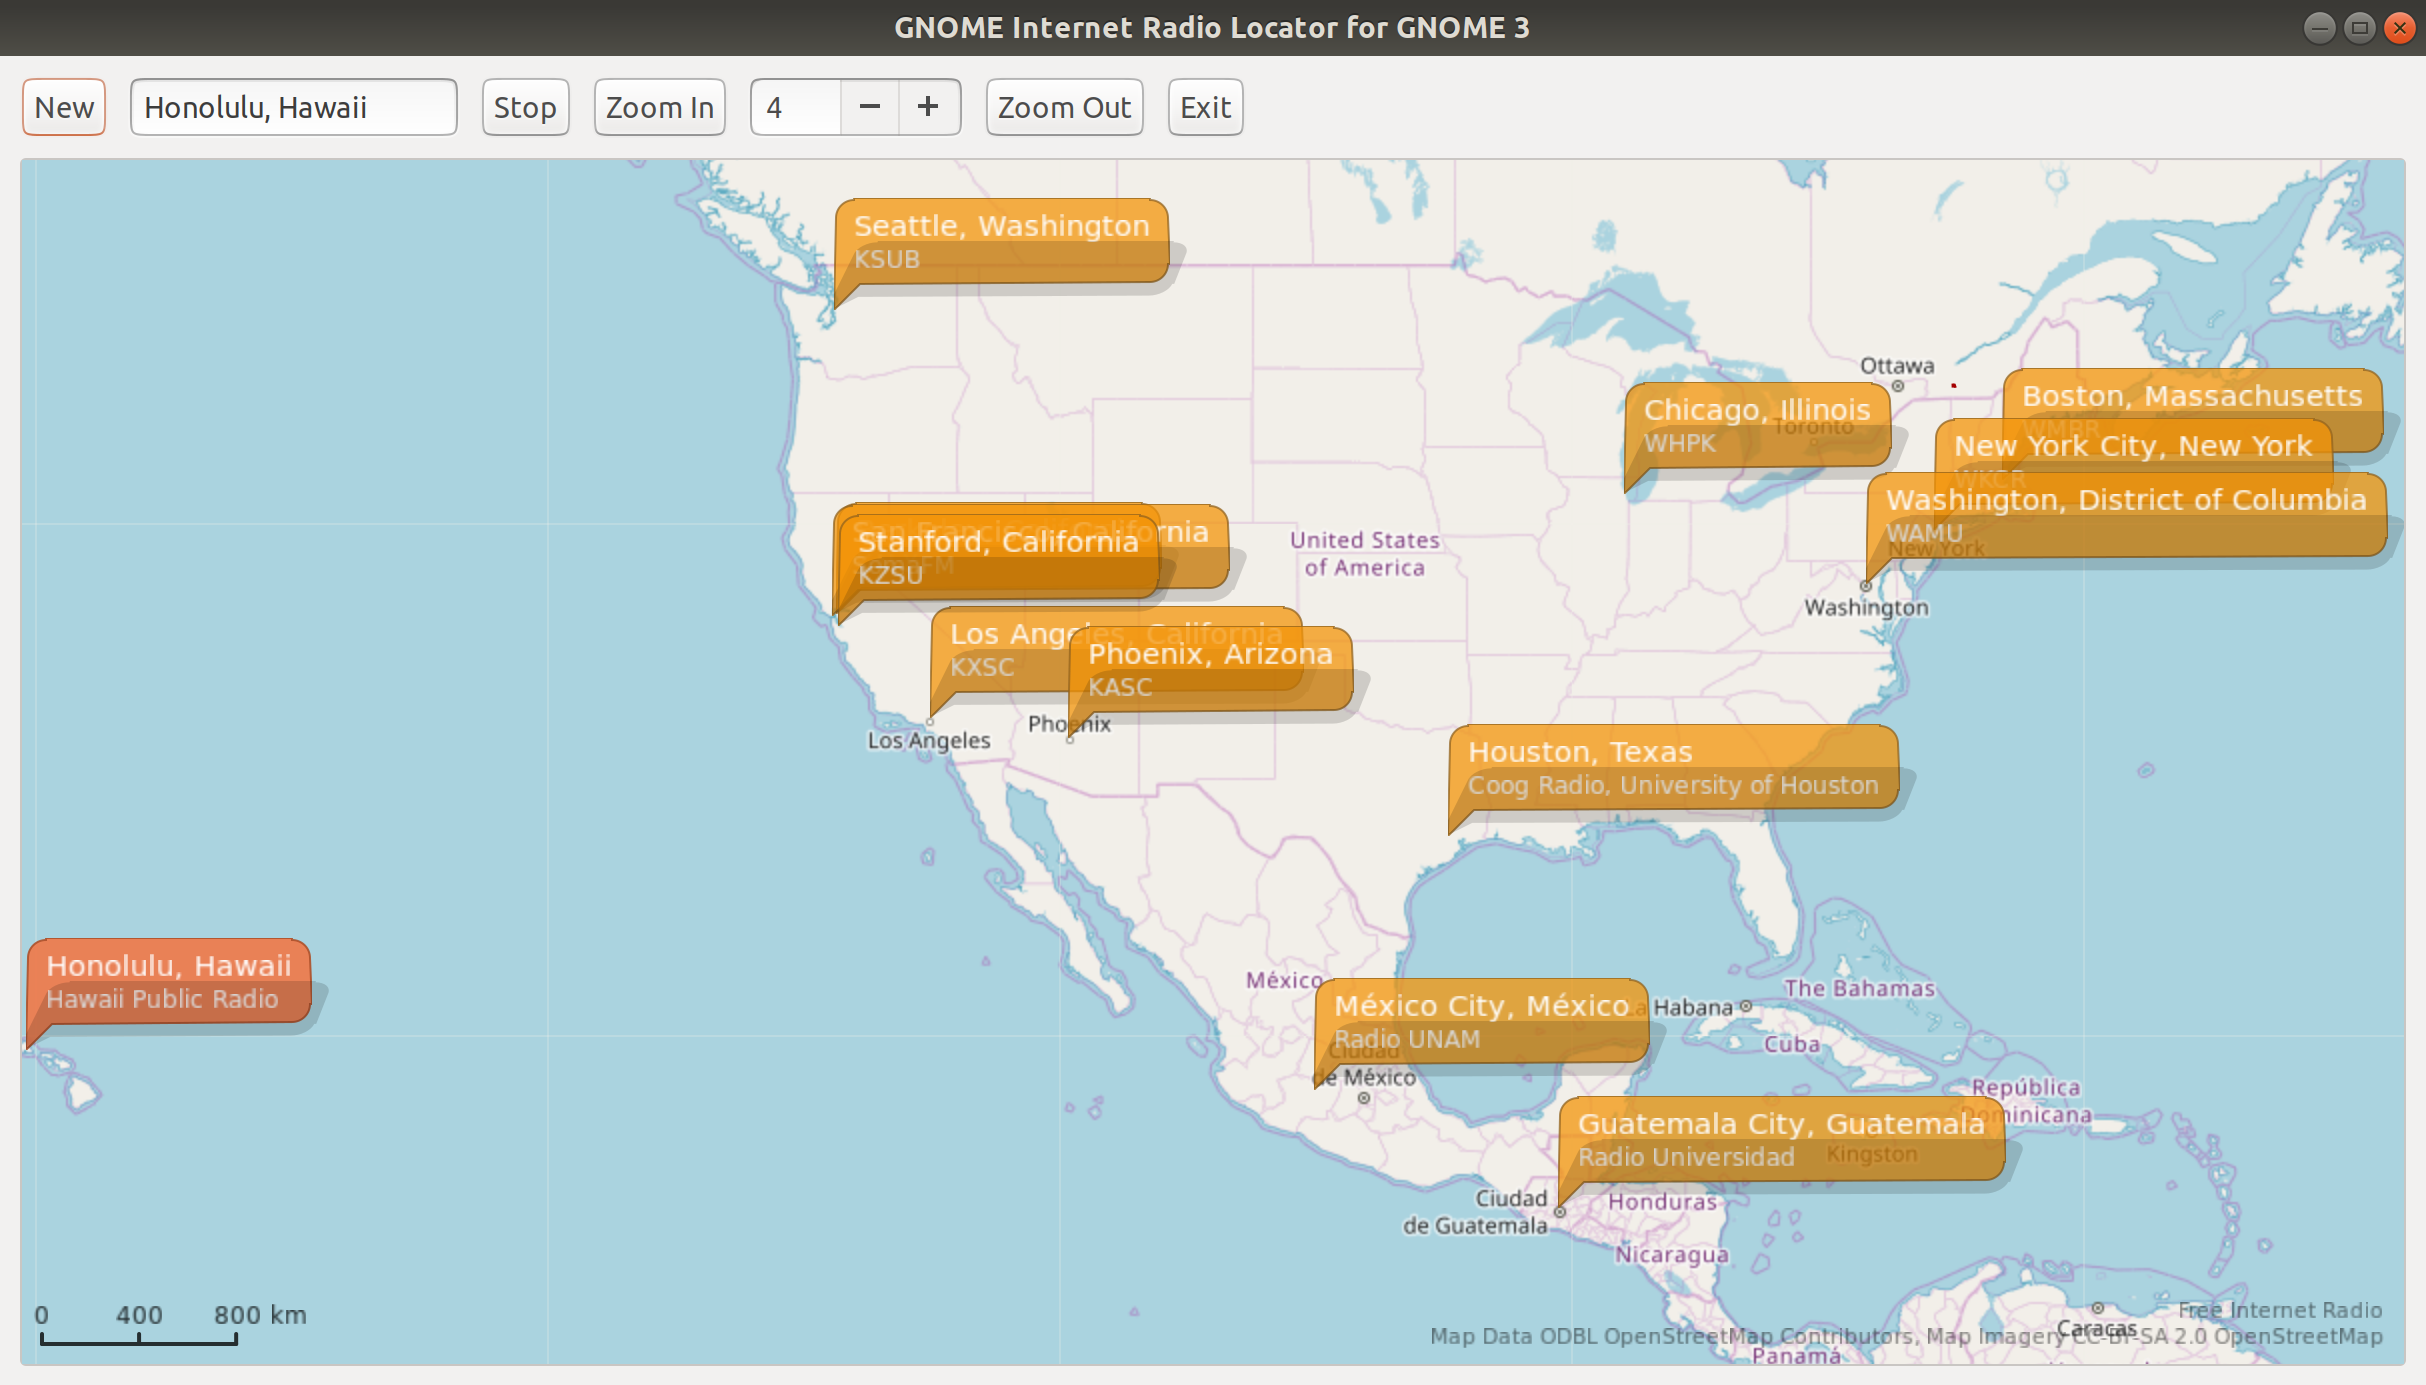
\includegraphics[width=0.6\hsize]{../data/screenshot.png}}

  {\blueem Screenshot of gnome-internet-radio-locator 2.1.1}

\end{center}

\slide{Legal stuff}

\begin{list1}
  \item Internet Radio stations in the U.S. need a broadcast license permit from the F.C.C.
    \begin{list2}
    \item Read gtk-internet-radio-locator/BROADCAST for some details on radio and music licensing
    \item \url{http://en.wikipedia.org/wiki/Broadcast_license}
    \item \url{https://www.dnalounge.com/backstage/webcasting.html}
    \end{list2}
  \item Personal Radio Stations can be set up using Icecast streaming server
    \begin{list2}
    \item Download Icecast from \url{http://www.icecast.org/} and add your station in \$HOME/.gnome-internet-radio-locator/gnome-internet-radio-locator.xml
    \end{list2}
  \item Only Internet radio stations with broadcast permit are included in gnome-internet-radio-locator
\end{list1}

\slide{Internet Radio Fairness Act}

\begin{list1}
\item Many Internet radio stations can't afford to pay royalty fee collection agencies
  \begin{list2}
  \item The American Society of Composers, Authors and Publishers (ASCAP)
  \item Broadcast Music, Inc. (BMI)
    \item Society of European Stage Authors and Composers (SESAC)
  \end{list2}
  \item New bill in support of Internet Radio introduced in U.S. Congress 2002:
  \begin{list2}
  \item \url{https://www.eff.org/Internet-Radio-Fairness-Act-Explanation}
  \item \url{http://en.wikipedia.org/wiki/Internet_Radio_Equality_Act}
  \end{list2}
\item EFF had a 2012 campaign in support of the Internet Radio Fairness Act
  \begin{list2}
  \item \url{https://www.eff.org/Internet-Radio-Fairness-Act-Explanation}
  \end{list2}
\item The IRFA bill may be reintroduced in U.S. Congress in 2019, but who knows?
\end{list1}

\slide{Email from Dr. Richard M. Stallman of FSF}

\begin{list1}
\item
  \begin{tiny}
\begin{verbatim}
    From: Richard Stallman <rms@gnu.org>
    Subject: Re: Internet Radio Fairness Act? (Re: It's your birthday)
    Date: Mon, 23 Mar 2015 22:43:25 -0400
    To: oka@oka.no

    [[[ To any NSA and FBI agents reading my email: please consider    ]]]
    [[[ whether defending the US Constitution against all enemies,     ]]]
    [[[ foreign or domestic, requires you to follow Snowden's example. ]]]

      > Regarding updating the LETTER included in GNOME Internet Radio Locator,
      > I don't know what to write/who to contact to promote Internet Radio
      > Fairness Act again in U.S. politics, except you.

    Ask people to contact their congressional representatives.

    Can you write a message to the public about this?

    -- 
    Dr Richard Stallman
    President, Free Software Foundation
    51 Franklin St
    Boston MA 02110
    USA
    www.fsf.org  www.gnu.org
    Skype: No way! See stallman.org/skype.html.
\end{verbatim}
  \end{tiny}
\end{list1}  

\slide{Questions?}

\begin{list1}
\item gnome-internet-radio-locator 2.1.1 is available here and now.
  \begin{list2}
  \item \begin{tiny}\url{http://download.gnome.org/sources/gnome-internet-radio-locator/2.1/gnome-internet-radio-locator-2.1.1.tar.xz}\end{tiny}
  \end{list2}
\item Debian 10 stable package
  \begin{list2}
  \item \begin{tiny}\url{https://www.gnome.org/~ole/debian/gnome-internet-radio-locator_2.1.1-1_i386.deb}\end{tiny}
  \end{list2}
\item Fedora 30 RPM
  \begin{list2}
  \item \begin{tiny}\url{https://www.gnome.org/~ole/fedora/RPMS/x86_64/gnome-internet-radio-locator-2.1.1-1.fc30.x86_64.rpm}\end{tiny}
  \end{list2}
\item Ubuntu 19.10 package
  \begin{list2}
  \item \begin{tiny}\url{https://www.gnome.org/~ole/ubuntu/gnome-internet-radio-locator_2.1.1-1_amd64.deb}\end{tiny}
  \end{list2}
\item Source repository
  \begin{list2}
    \item \url{git://gitlab.gnome.org/GNOME/gnome-internet-radio-locator}
    \item \url{https://gitlab.gnome.org/GNOME/gnome-internet-radio-locator}
    \item \url{ssh://$USERNAME@gitlab.gnome.org/GNOME/gnome-internet-radio-locator}
  \end{list2}
\end{list1}

\slide{\LaTeX{} source code for this presentation}

\url{https://gitlab.gnome.org/GNOME/gnome-internet-radio-locator/plain/talk/GC2019.tex}

\slide{GNOME Wiki page for GNOME Radio}

\url{https://wiki.gnome.org/Apps/Radio}

\end{document}
